\chapter{INTRODUCTION}
\label{chap:intro}



\section{Motivation}

We want to learn graph from data to encode relationships between entities. These entities and relationships can be represented using nodes and edges of the graph. The edge weight corresponds to the strength of connection between two nodes. The learned graphs have numerous applications in Graph Neural Networks (GNNs), graph signal processing, classification, prediction, smoothing, structural inference etc. With the advent of GNNs, learning graphs from data holds tremendous potential with applications such as node classification, pairwise node classification etc. Fig~\ref{fig:graph-from-brain-data} shows the time series data samples observed from different parts in the brain. These signals can represent the neural activity of a part of the brain over time. If we can learn graph from data, we can capture the useful relationships between these nodes.

\begin{center}
	\begin{figure}[htpb]
		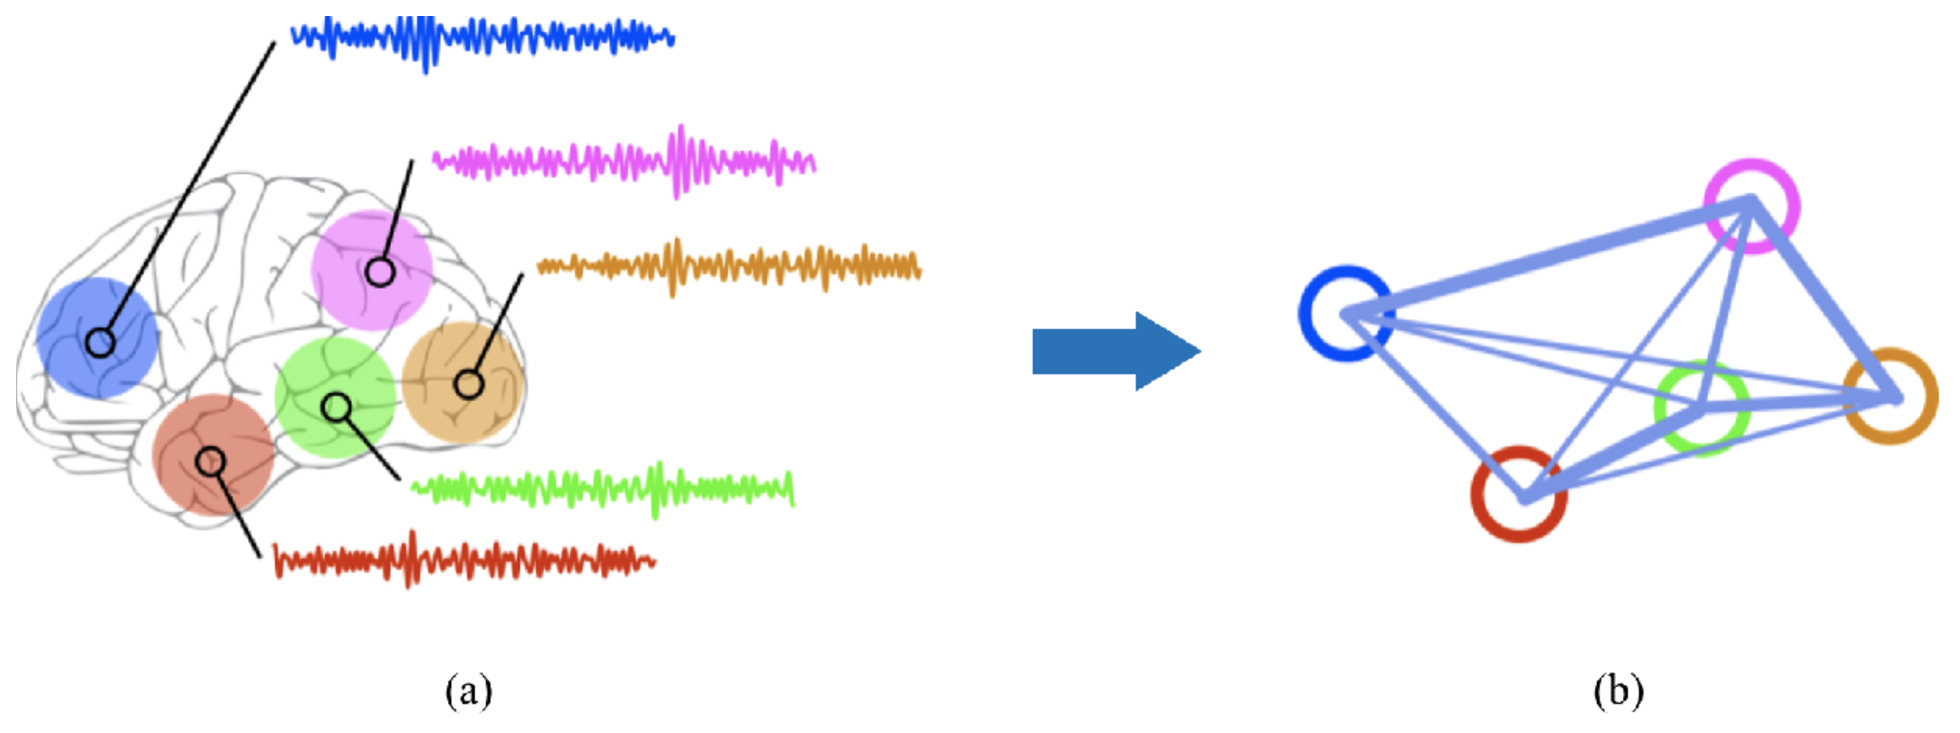
\includegraphics[scale=0.45]{Pictures/dong.eps}
		\caption{Learning graph from brain data signals. Image src: \cite{dong2019learning}  }
		\label{fig:graph-from-brain-data}
	\end{figure}
\end{center}

Our goal is to learn a graph $\mathcal{G} = (\mathcal{V}, \mathcal{E}, W)$, where $\mathcal{V} = {1, 2, ..., p}$ is the node set consisting of $p$ nodes corresponding to the entities and $\mathcal{E}={(1,2), (1,3), ...}$ is the edge set with $|\mathcal{E}|$ number of edges representing the relationships between these entities. The weight matrix $W$ represents the edge weights denoting the strength of these relationships. For the sake of simplicity, we restrict ourselves to a class of Probabilistic Graphical Models (PGMs) called the Gaussian Graphical Models (GGMs). The assumption of gaussianity is not too restricting in the sense that if we have large number of samples, the distribution converges into gaussian distribution due to the central limit theorem. Fig~\ref{fig:graph-from-data} pictorially depicts our goal of learning graph from $\mathbb{R}^{n \times p} $ data.

\begin{center}
	\begin{figure}[htpb]
		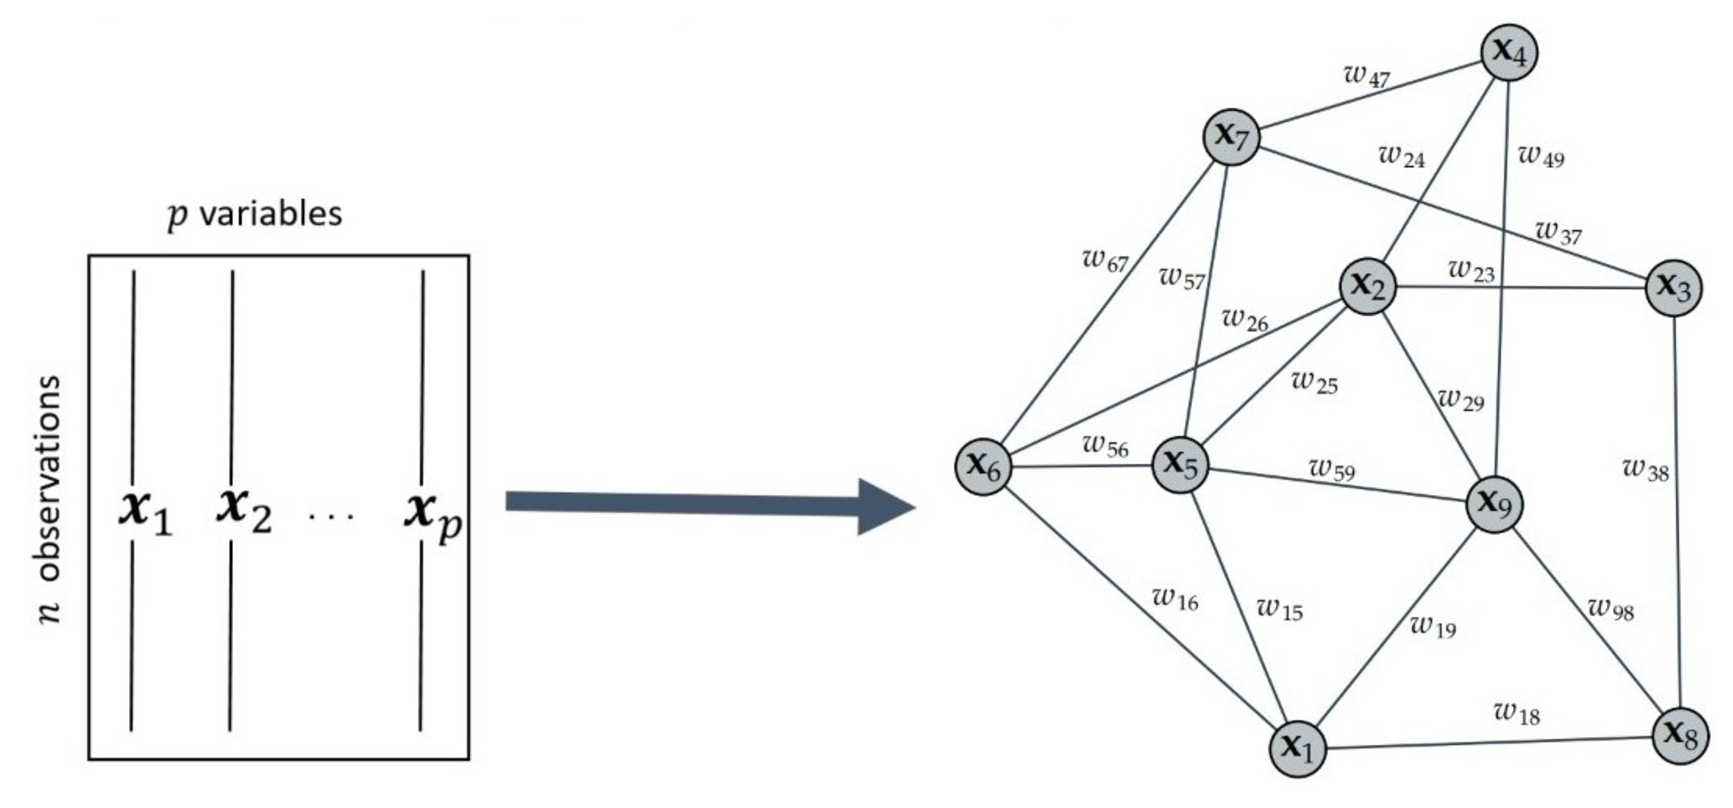
\includegraphics[scale=0.45]{Pictures/data.eps}
		\caption{Learning graph structure from data  }
		\label{fig:graph-from-data}
	\end{figure}
\end{center} 

\section{Gaussian Graphical Models}
Gaussian Graphical Models are essentially multivariate gaussian distributions. Consider the following density of multivariate gaussian distribution:
\begin{equation}
p(\mathbf{x} \mid \mu, \Sigma)=\frac{1}{(2 \pi)^{n / 2}|\Sigma|^{1 / 2}} \exp \left(-\frac{1}{2}(\mathbf{x}-\mu)^{\top} \Sigma^{-1}(\mathbf{x}-\mu)\right)
\end{equation}
Let $\mathbf{\Theta = \Sigma^{-1}}$, also known as the precision matrix. We have $n$ i.i.d. samples from this multivariate normal distribution such that $\mathbf{X} = \left\{\mathbf{x}^{(i)} \sim \mathcal{N}\left(\mathbf{0}, \Sigma\right)\right\}_{i=1}^{n}$. The graphical model aspect comes from the fact that given any pair of nodes $\mathbf{x_i}$ and $\mathbf{x_j}$ and a set of nodes $\mathbf{x_S}$, then $\mathbf{x_i}$ is conditionally independent of $\mathbf{x_j}$ given $\mathbf{x_S}$, thus following the Markov property. Mathematically, $$\mathbf{x_i \perp \!\!\! \perp  x_j \mid x_{S}}$$ There is an edge between nodes $\mathbf{x_i}$ and $\mathbf{x_j}$ if and only if $\mathbf{\Theta_{ij} = (\Sigma^{-1})_{ij} \ne 0}$. Therefore we can easily construct the graph if we know the entries of $\mathbf{\Theta}$ as it will directly give the edges between nodes. Therefore the problem of graph structure learning essentially boils down to learning the precision or the inverse covariance matrix $\mathbf{\Theta}$.

\subsection{GGM optimization problem} 
GGMs are often formulated in the Maximum Likelihood Estimation (MLE) settings \citep{uhler2017gaussian}. Given the data samples, $\mathbf{X}=\left\{\mathbf{x}^{(i)} \in \mathbb{R}^{p}\right\}_{i=1}^{n}$, the log likelihood for GGMs can be computed as follows:
\begin{eqnarray}
	\begin{aligned}
		\ell(\mu, \Sigma) & \propto-\frac{n}{2} \log \operatorname{det}(\Sigma)-\frac{1}{2} \sum_{i=1}^{n}\left(\mathbf{x}^{(i)}-\mu\right)^{T} \Sigma^{-1}\left(\mathbf{x}^{(i)}-\mu\right) \\
		&=-\frac{n}{2} \log \operatorname{det}(\Sigma)-\frac{1}{2} \operatorname{Tr}\left(\Sigma^{-1}\left(\sum_{i=1}^{n}\left(\mathbf{x}^{(i)}-\mu\right)\left(\mathbf{x}^{(i)}-\mu\right)^{T}\right)\right) \\
		&=-\frac{n}{2} \log \operatorname{det}(\Sigma)-\frac{n}{2} \operatorname{Tr}\left(S \Sigma^{-1}\right)-\frac{n}{2}(\bar{\mathbf{x}}-\mu)^{T} \Sigma^{-1}(\bar{\mathbf{x}}-\mu)
	\end{aligned}
\end{eqnarray}
where $\bar{\mathbf{x}}$ is the sample mean and $\mathbf{S}$ is the Sample Covariance Matrix (SCM) defined as: 
$$
\mathbf{S}= \frac{1}{n} \mathbf{X}\mathbf{X}^T =\frac{1}{n} \sum_{i=1}^{n}\left(\mathbf{x}^{(i)}\right)\left(\mathbf{x}^{(i)}\right)^{\top}
$$

Maximizing the above log-likelihood to formulate an optimization problem over the precision matrix $\mathbf{\Theta}$ we get the following optimization objective:
\begin{equation}
\mathbf{	\underset{\Theta \succeq 0}{\operatorname{maximize}} \log \operatorname{det}(\Theta)-\operatorname{Tr}(\Theta S)-\alpha h(\Theta)}
\end{equation}
where an additional term $h(\Theta)$ is introduced to regularize $\Theta$ and $\alpha$ is the regularization parameter. Choice of $h(.)$ is dependent on the objective of formulation. One simple choice can be $l1$-regularization \citep{friedman2008sparse}.
